%%%%%%%%%%%%%%%%%%%%%%%%%%%%%%%%%%%%%%%%%%%%%%%%%%%%%%%%%%%%%%%%%%%%%%%%%%%%%%%%
\chapter{Partitioning Algorithms}
\label{ch:part}
%%%%%%%%%%%%%%%%%%%%%%%%%%%%%%%%%%%%%%%%%%%%%%%%%%%%%%%%%%%%%%%%%%%%%%%%%%%%%%%%

We mentioned earlier that the MLP is usually approached in two phases:
placement and re-embedding. The placement, however, is sometimes
preceded by a \emph{partitioning} phase, which breaks the problem into
smaller sub-problems that are easier to manage. This is especially
helpful for placement algorithms with non-linear time or space
complexities that are otherwise unable to handle very large chips.

A partitioning algorithm divides the set of probes $\mathcal{P}$ into smaller
subsets, and assigns them to defined regions of the chip. Each region can then
be treated as an independent chip (and processed by a placement algorithm) or
recursively partitioned. Linear-time placement algorithms may also benefit from
a partitioning since probes with similar embeddings are typically assigned to
the same region (Row-Epitaxial, for instance, is more likely to find good
candidates for filling a spot).

We describe four partitioning algorithms: 1-Dimensional Partitioning,
2-Dimen\-sional Partitioning, Centroid-based Quadrisection (CQ), and
Pivot Partitioning (PP). Like placement algorithms, they assume that
an initial (left-most, right-most, synchronous or otherwise
pre-computed) embedding of the probes is given. Pivot Partitioning is
the only algorithm that modifies these embeddings.  As we shall see,
1-D and 2-D Partitioning generate a few masks with extremely few
conflicts, leaving the remaining masks with high levels of conflicts
that are difficult to handle. CQ and PP offer a more uniform
optimization over all masks. Results of \citet{Carvalho2006} indicate
that PP produces better layouts than CQ on large chips.

Partitioning is a compromise in solution quality since it restricts
the space of solutions and may lead to conflicts at partition borders.
However, it can improve solution quality in practice when the
placement algorithm cannot handle large regions well. It is not
advisable to perform too many levels of partitionings because smaller
sub-regions mean less freedom for optimization during placement. The
right balance depends on both the placement algorithm and the
partitioning algorithm.


\section{1-Dimensional Partitioning}
\label{sec:part_1d}

1-Dimensional Partitioning divides the set of probes based on the state of
their embeddings at a particular synthesis step. It starts by creating two
subsets of $\mathcal{P}$:
%%
\[
\mathcal{P}_0 = \{ p_k \in \mathcal{P} | \eps_{k,1} = 0 \},
\qquad
\mathcal{P}_1 = \{ p_k \in \mathcal{P} | \eps_{k,1} = 1 \}.
\]

In other words, $\mathcal{P}_0$ contains all probes whose embeddings are
unproductive during the first synthesis step, whereas $\mathcal{P}_1$
contains the probes with productive embeddings. The chip is then
divided into two horizontal bands, proportionally to the number of probes in
$\mathcal{P}_0$ and $\mathcal{P}_1$, so each band accommodates one subset
of $\mathcal{P}$.

This procedure is recursively applied to each band, using the the next
synthesis steps to further divide each subset of probes. For
instance, the following subsets of $\mathcal{P}_0$ and
$\mathcal{P}_1$ are created during step $t=2$:
%%
\[
\mathcal{P}_{00} = \{ p_k \in \mathcal{P}_0 | \eps_{k,2} = 0 \},
\qquad
\mathcal{P}_{01} = \{ p_k \in \mathcal{P}_0 | \eps_{k,2} = 1 \},
\]
\[
\mathcal{P}_{10} = \{ p_k \in \mathcal{P}_1 | \eps_{k,2} = 0 \},
\qquad
\mathcal{P}_{11} = \{ p_k \in \mathcal{P}_1 | \eps_{k,2} = 1 \}.
\]

\begin{figure}\centering
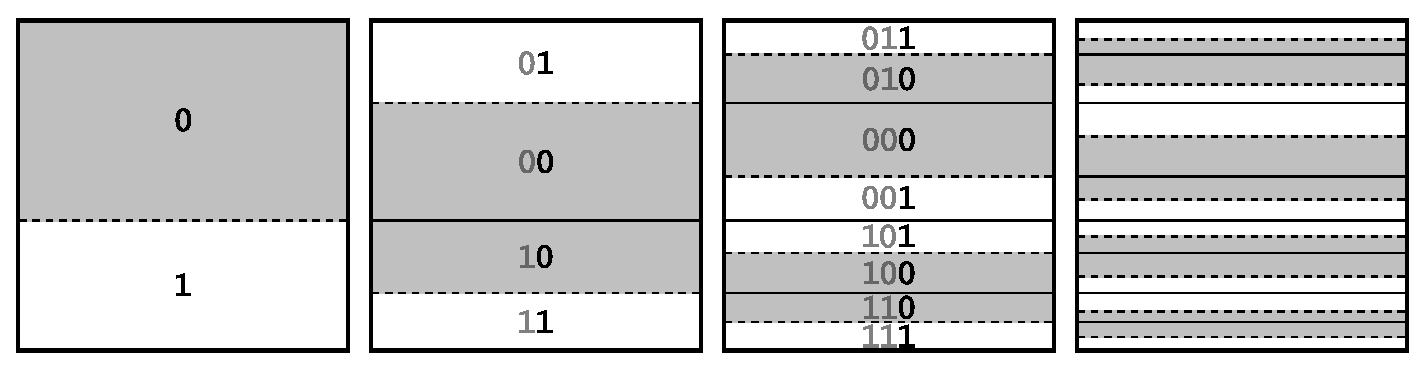
\includegraphics[width=\textwidth]{1dpart.eps}
\caption{\label{fig:1dpart}%
  First four levels of 1-Dimensional Partitioning. Dashed lines show the
  divisions performed in each step; solid lines indicate regions delimited in
  previous steps (there are no border conflicts between spots separated by
  solid lines). Masked (shaded) regions are labeled ``0'',
  unmasked (white) regions are labeled ``1''. This labeling forms
  a Gray code (shown in the first three steps only).}
\end{figure}


The next assignments of subsets to the upper or lower band of their regions
are made in such a way that regions with the same ``state'' --- productive
(unmasked) or unproductive (masked) --- are joined as far as
possible, resulting in masks that consist of alternating layers of masked and
unmasked spots. This process is illustrated in Fig.~\ref{fig:1dpart}, where at
each step~$t$, a band is labeled ``0'' when its embeddings are unproductive,
and ``1'' when its embeddings are productive. The resulting binary numbers
from top to bottom form a Gray code, i.e., two successive numbers differ in
only one bit.

The Gray code highlights an interesting property of 1-D Partitioning.
After $d$~levels of partitionings (based on steps $1$ to $d$), the
embeddings of any two immediate neighbors differ among the first
$d$~steps in at most one step.  As a result, masks $M_1 \dots M_d$
exhibit a layered structure that effectively reduces border conflicts.

Unfortunately, the Gray code is disrupted as soon as a region cannot be divided
(because all probes of that region are, for instance, masked at a particular
step). This will certainly happen as several binary numbers are unlikely to be
substrings of embeddings (think of, for example, a long run of zeros).

Moreover, 1-D Partitioning can optimize only a limited number of masks
because the sub-regions soon become too narrow to be further divided. The
maximum \emph{partitioning depth} $d_{max}$ is primarily limited by the number
of rows in the chip. In practice, since regions are likely to be unevenly
divided, $d_{max}$ varies between regions. The algorithm can also be configured
to stop partitioning a region once its dimensions drop below a given threshold.

1-D Partitioning is easier to implement if the partitionings always produce
rectangular regions (i.e., splitting a row between two regions is not allowed).
In order to force an exact division of a region, however, it might be necessary
to move a few probes from one subset of probes to the other one.

For example, imagine that a chip with $|\mathcal{P}| = 900$ probes, $n_r = 30$
rows and $n_c = 30$ columns is to be partitioned based on the state of the
embeddings at the first synthesis step, resulting in sub-sets $\mathcal{P}_0$
and $\mathcal{P}_1$ with, say, 638 and 262 probes, respectively. The chip must
thus be divided into two sub-regions, the upper one containing $[30 \cdot
638/900]=21$ rows and the lower one with $[30 \cdot 262/900]=9$ rows ($[x]$ is
$x$ rounded to the nearest integer). The problem is that the upper region then
contains $21 \cdot 30 = 630$ spots but it has to accommodate 638 probes,
whereas the lower region contains $9 \cdot 30 = 270$ spots but only 262
probes. The solution is to (arbitrarily) move 8 probes from $\mathcal{P}_0$ to
$\mathcal{P}_1$, which, results in some imperfections in the layers
of the corresponding mask (a few masked spots in a region of unmasked spots,
for instance).

\section{2-Dimensional Partitioning}
\label{sec:part_2d}

%%%
\begin{figure}\centering
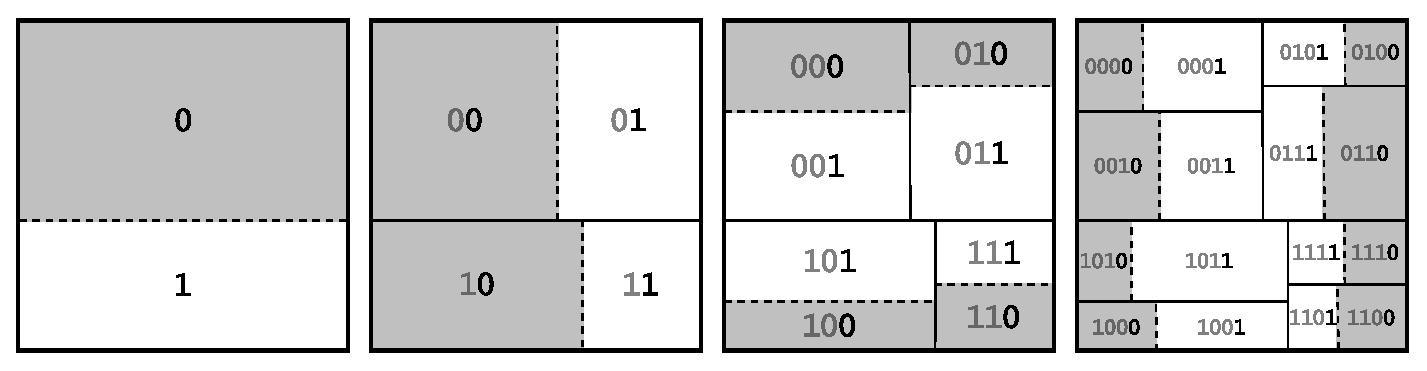
\includegraphics[width=\textwidth]{2dpart.eps}
\caption{\label{fig:2dpart}%
  First four levels of 2-Dimensional Partitioning. Dashed lines show
  the divisions performed in each step; solid lines indicate regions
  delimited in previous steps. Masked regions are labeled with ``0'',
  unmasked regions with ``1''; this labeling forms an approximation to
  a two-dimensional Gray code.}%
\end{figure}
%%%

The 2-Dimensional Partitioning algorithm extends the idea of 1-D
Partitioning to two dimensions, with the potential of optimizing twice
as many masks. The algorithm is similar: $\mathcal{P}$ is divided into
subsets based on the state of the embeddings at a particular
synthesis step. The difference is that 2-D Partitioning alternates
horizontal and vertical divisions of regions, and that the assignments
of probes to regions obey a two-dimensional Gray code
(Fig.~\ref{fig:2dpart}).

In a 2-D Gray code, two neighboring numbers differ in at most one
bit.  Thus, regions whose embeddings are at the same state (productive or
unproductive) are joined as far as possible.

If regions were always equally divided, 2-D Partitioning would have
the same property as 1-D Partitioning: After $d$~levels of
partitionings (based on steps $1$ to $d$), the embeddings of any two
immediate neighbors would differ among the first $d$ steps in at most
one step. However, this is not always the case since 2-D Partitioning
is likely to create regions with different dimensions, forcing some
regions to share a border with more than its four natural neighbors
(for example, region ``1100'' in Fig.~\ref{fig:2dpart} borders with
``0101'' and ``1111'').

So far we have described both 1-D and 2-D Partitionings using the
state of the first $d$ synthesis steps to divide the set of probes.
The result of this approach is that, while the first masks are
optimized, the remaining masks are left with high levels of border
conflicts; we call this a \emph{left-most mask optimization}.

However, a defect in the middle of the probe is more harmful than in
its extremities, so it is more important to optimize the central masks,
which synthesize the middle bases. Thus we
partition the chip based on the following sequence
of synthesis steps, assuming that $T$ is even and $d$ is odd: $T/2,
(T/2)\pm 1, (T/2)\pm 2, \dots, (T/2)\pm\lfloor d/2\rfloor$; we call
this a \emph{centered mask optimization}.

For left-most optimization, it makes sense to embed the probes in a
left-most fashion in order to reduce conflicts in the last masks
(which are not optimized by the partitioning); the left-most
embeddings reduce the number of unmasked spots in the last steps,
resulting in masks that largely consist of masked spots. Similarly,
centered mask optimization produces better results with \emph{centered
  embeddings}. A centered embedding is constructed by shifting a
left-most embedding to the right so that the number of masked steps to
the left of the first productive step approximately equals the number
of masked steps to the right of the last productive step.

%%%
\begin{figure}\centering
%%
\begin{picture}(335,150)\footnotesize{
  \put(0,0){\makebox(335,150){
    %GNUPLOT: LaTeX picture with Postscript
    \begin{picture}(0,0)%
    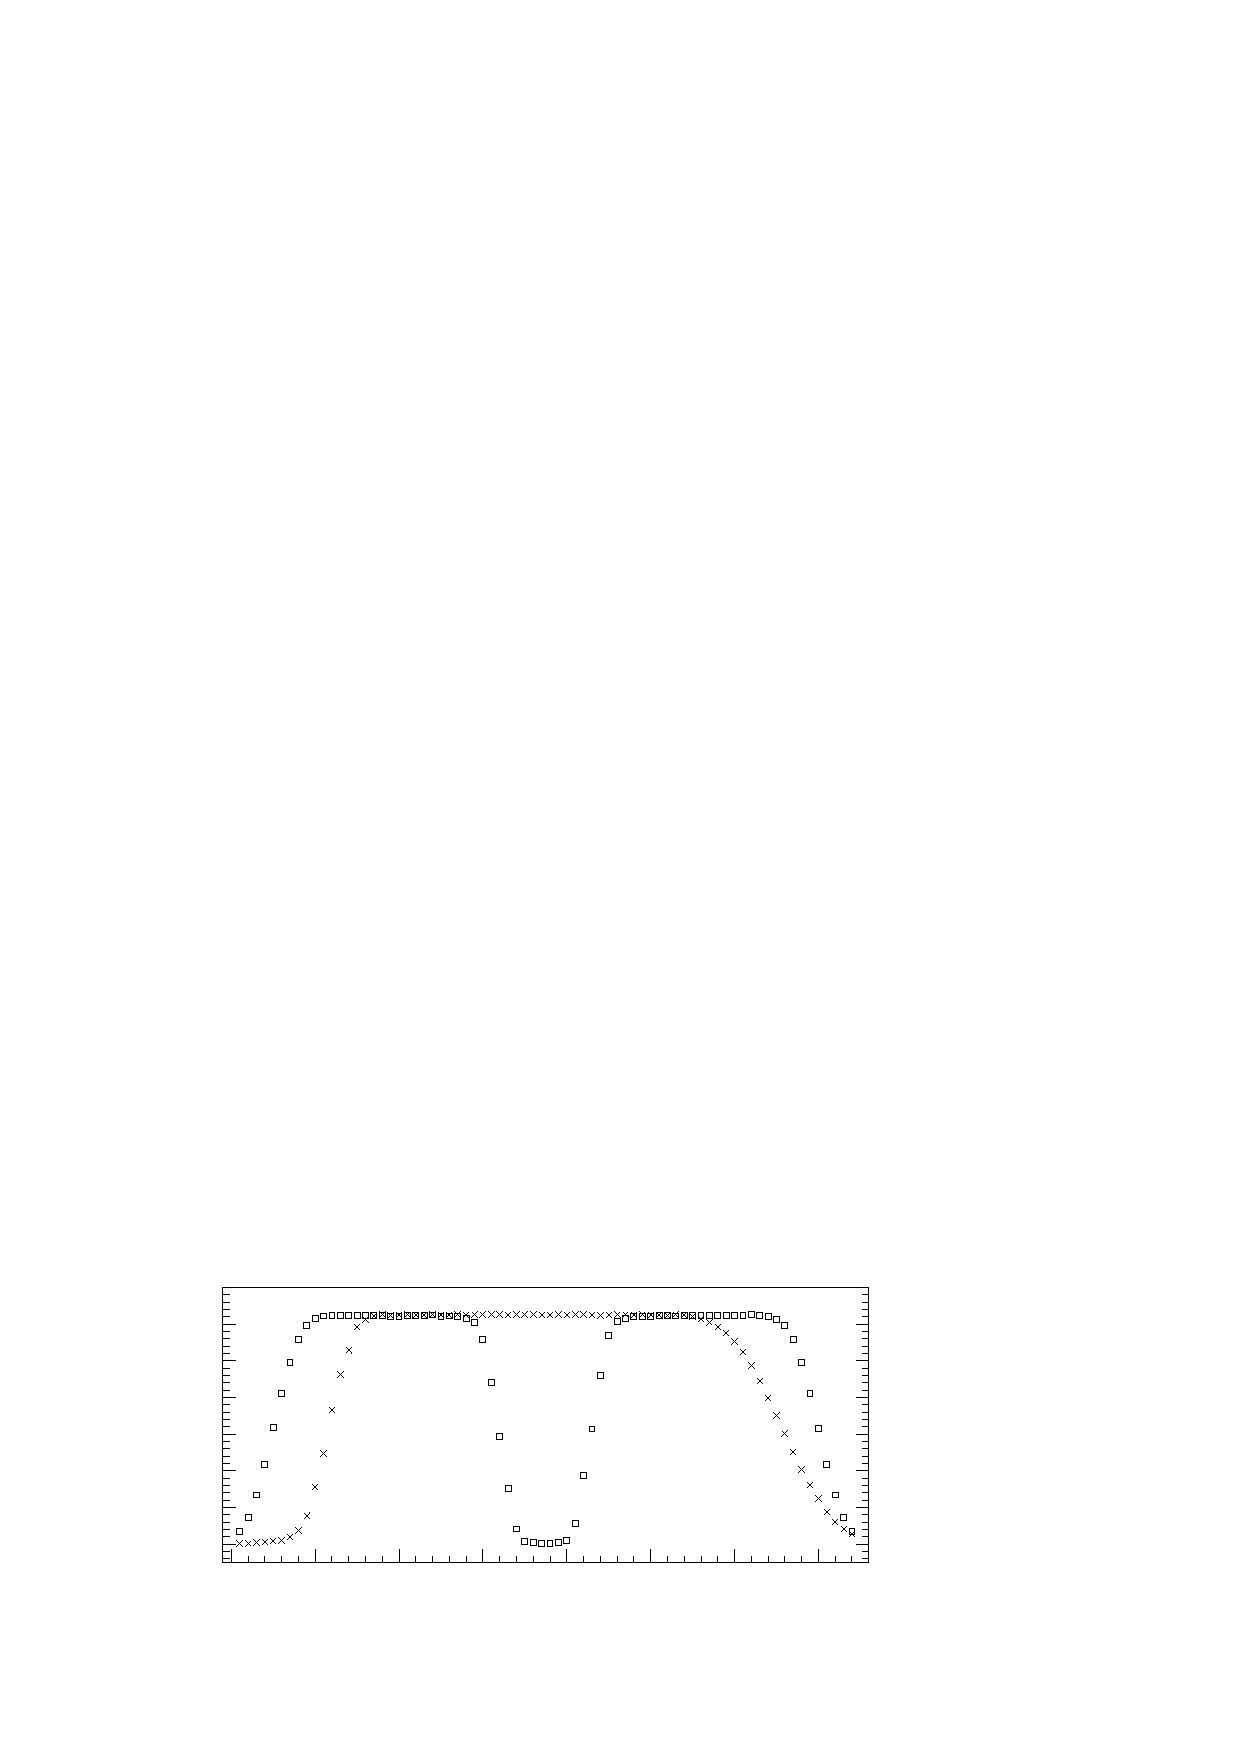
\includegraphics{2dpart_bl/2dpart_bl}%
    \end{picture}%
    \begingroup
    \setlength{\unitlength}{0.0200bp}%
    \begin{picture}(18000,8100)(0,0)%
    \put(1500,1440){\makebox(0,0)[r]{\strut{} 0}}%
    \put(1500,2320){\makebox(0,0)[r]{\strut{} 0.1}}%
    \put(1500,3200){\makebox(0,0)[r]{\strut{} 0.2}}%
    \put(1500,4080){\makebox(0,0)[r]{\strut{} 0.3}}%
    \put(1500,4960){\makebox(0,0)[r]{\strut{} 0.4}}%
    \put(1500,5840){\makebox(0,0)[r]{\strut{} 0.5}}%
    \put(1500,6720){\makebox(0,0)[r]{\strut{} 0.6}}%
    \put(1500,7600){\makebox(0,0)[r]{\strut{} 0.7}}%
    \put(1951,500){\makebox(0,0){\strut{} 0}}%
    \put(3964,500){\makebox(0,0){\strut{} 10}}%
    \put(5977,500){\makebox(0,0){\strut{} 20}}%
    \put(7990,500){\makebox(0,0){\strut{} 30}}%
    \put(10003,500){\makebox(0,0){\strut{} 40}}%
    \put(12016,500){\makebox(0,0){\strut{} 50}}%
    \put(14029,500){\makebox(0,0){\strut{} 60}}%
    \put(16042,500){\makebox(0,0){\strut{} 70}}%
    \end{picture}%
    \endgroup
  }}
}\end{picture}
%%
%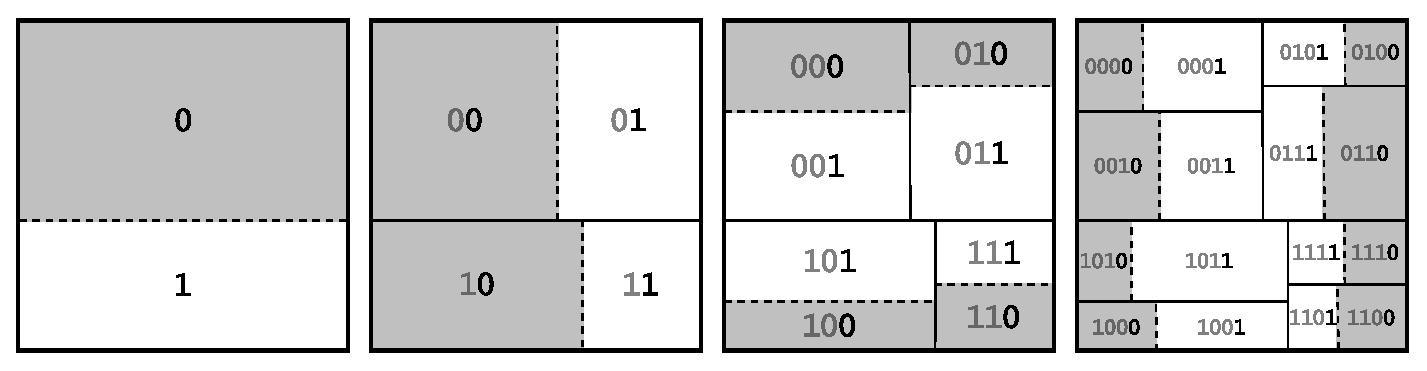
\includegraphics[width=\textwidth]{2dpart.eps}
\caption{\label{fig:2dpart_bl}%
  Normalized border length (on the y-axis) per masking step (on the x-axis) of
  a layout produced by 2-Dimensional Partitioning for a $1\,000 \times 1\,000$
  chip with random probe sequences (embedded in the standard 74-step Affymetrix
  deposition sequence). Partitioning stops when a region becomes smaller than
  $64 \times 64$; Row-Epitaxial is used for the placement. ({\tiny $\times$})
  Left-most mask optimization with left-most embeddings; ({\tiny $\Box$})
  centered mask optimization with centered embeddings.}
\end{figure}
%%%

Fig.~\ref{fig:2dpart_bl} shows the results of 2-D Partitioning on a
$1\,000\times 1\,000$ chip with both optimizations. For left-most mask
optimization, we obtain a normalized border length of 33.89 (up to
approximately 0.6 per step). For centered mask optimization, the normalized
border length improves slightly to 33.59. The average conflict index (not
shown in the figure) for left-most mask optimization is 571.8; for centered
mask optimization, it improves considerably to 383.5 because of the higher
weight of the middle bases.


\section{Centroid-based Quadrisection}
\label{sec:part_cq}

\begin{figure}\centering
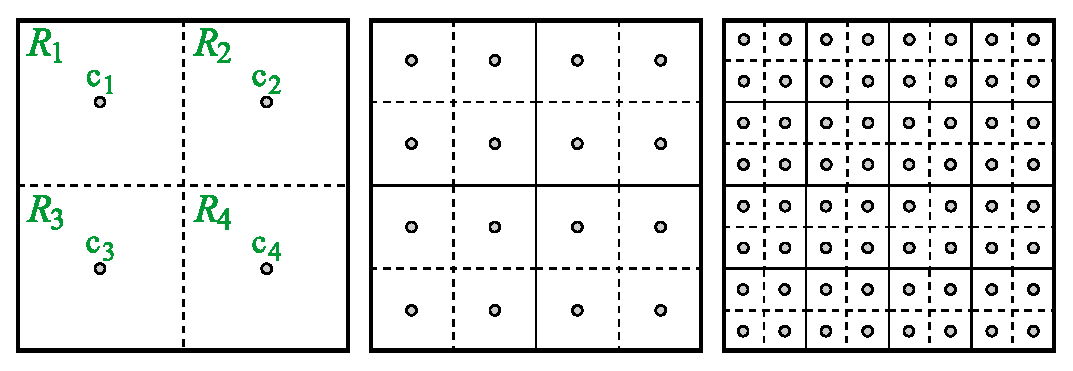
\includegraphics[width=\textwidth]{quadrisect.eps}
\caption{\label{fig:quadrisect}%
  First three levels of Centroid-base Quadrisection Partitioning. Dashed lines
  show the divisions performed in each step; solid lines indicate regions
  delimited in previous steps. The centroids of each partition $R_1 \dots R_4$
  are represented by small circles (labeled with $q_1 \dots q_4$ in the first
  step).}
\end{figure}

Centroid-based Quadrisection or CQ \citep{Kahng2003a} employs a
different criterion for dividing the set of probes and a different
approach for partitioning. At each iteration, a region $R$ is
quadrisectioned into $R_1$, $R_2$, $R_3$, and $R_4$. Each sub-region
$R_i$ is associated with a selected probe $p_{c_i}\in \mathcal{P}$,
called \emph{centroid}, that is used to guide the assignment of the
remaining probes to the sub-regions.

A centroid is a representative of its region; it should symbolize the
``average embedding'' in that region. The remaining probes $p_k \in
\mathcal{P} \setminus \{p_{c_1},p_{c_2},p_{c_3},p_{c_4}\}$ are
compared to each centroid and assigned to the sub-region $R_i$ whose
centroid's embedding $\eps_{c_i}$ has minimum $H(k,c_i)$, where
$H(k,k')$ is the Hamming distance between the embeddings $\eps_k$ of
$p_k$ and $\eps_{k'}$ of $p_{k'}$ (i.e., the number of steps in which
$\eps_k$ and $\eps_{k'}$ differ).

In order to improve the clustering of similar probes, the four
centroids should be very different from each other. The following
heuristic is used: First, a probe index $c_1$ is randomly selected
from $\{1,\dots,|\mathcal{P}|\}$.  Then, a probe index $c_2\neq c_1$
maximizing $H(c_2,c_1)$ is selected.  Similarly, $c_3$ maximizing
$H(c_3,c_1) + H(c_3,c_2)$ and $c_4$ maximizing $H(c_4,c_1) +
H(c_4,c_2) + H(c_4,c_3)$ are selected.  The assignment of centroids to
the quadrisections of the chip is arbitrary.

In order to recover from a possibly bad choice of centroids, one can
use a ``multi-start heuristic'', running the centroid selection
procedure several times (using different ``seeds'' for $c_1$), and
keeping those that lead to the best partitioning (partitioning quality
is measured by the sum of Hamming distances of probe embeddings to
their corresponding centroid embeddings).

The partitioning continues recursively until a pre-defined depth has been
reached.

CQ was developed for border length minimization, but can be adapted
for conflict index minimization by using the \emph{conflict index
  distance} $C(k,k')$ instead of the Hamming distance $H(k,k')$
between the embeddings $\eps_k$ and $\eps_{k'}$.

\section{Pivot Partitioning: Merging partitioning and re-embedding}
\label{sec:part_pp}

Pivot Partitioning or PP \citep{Carvalho2006} is, to a certain extent,
similar to CQ: Sub-regions are recursively associated with special
probes $p_{c_i}$, here called \emph{pivots} instead of centroids, that
are used to guide the assignment of the other probes to the
sub-regions.  The main differences between PP and CQ are as follows.

Instead of quadrisectioning the chip, PP creates sub-regions by
alternating horizontal and vertical divisions (like 2-D Partitioning).
The advantage is that regions are divided proportionally to the size
of each subset of probes, so they are not required to have the same
size. Furthermore, for each partitioning level, only two pivots need
to be selected.

Another distinction is motivated by the fact that different probes
have different numbers of embeddings, ranging from a single one to
several millions.  Probes with more embeddings can more easily adapt
to the other probes, that is, they are more likely to have an
embedding with fewer conflicts to fill a particular spot than a probe
that has only a limited number of embeddings. For this reason, PP uses
probes with a single embedding (or few embeddings) as pivots, and
chooses the other probes' embeddings and region assignments accordingly.

Indeed, the most important feature of PP is the simultaneous embedding and
assignment of probes to sub-regions. Let $M(k,c_i)$ denote the minimum
conflict index distance $C(k,c_i)$, as defined in~(\ref{eq:ci_dist}), over all
embeddings of $p_k$; we call it the \emph{minimum conflict index distance}
between probes $p_k$ and $p_{c_i}$. It can be efficiently computed with a
variant of the OSPE algorithm that ignores the location of the probes and the
distance-dependent weights $\gamma$. Now, a non-pivot probe $p_k$ is assigned
to the region $R_i$ whose pivot $p_{c_i}$ has minimum $M(k,q_i)$ over $i=1,2$.
Pivot Partitioning continues recursively up to a pre-defined depth. Finally,
each probe is embedded to minimize conflicts with its assigned pivot.
